\chapter{Reactive Systems}

\section{Reactive Manifesto}

Organizations working in disparate domains are independently discovering patterns for building software that look the same. These systems are more robust, more resilient, more flexible and better positioned to meet modern demands.

These changes are happening because application requirements have changed dramatically in recent years. Only a few years ago a large application had tens of servers, seconds of response time, hours of offline maintenance and gigabytes of data. Today applications are deployed on everything from mobile devices to a cloud-based clusters running thousands of multi-core processors. Users expect milliseconds response times and 100\% up-time. Data is measured in petabytes. Today's demands are simply not met by yesterday's software architecture.

A coherent approach to systems architecture is needed, and all necessary aspects are already recognized individually. Systems must be (Figure \ref{fig:responsive}):
\begin{itemize}
    \item Responsive;
    \item Resilient;
    \item Elastic;
    \item Message-Driven.
\end{itemize}
Systems that have all of the above characteristics are called Reactive Systems. They are more:
\begin{itemize}
    \item Flexible;
    \item Loosely-coupled;
    \item Scalable.
\end{itemize}
Because of that these ones are easier to develop and amenable to change. They are significantly more tolerant of failure and when failure does occur they meet it with elegance rather than disaster.  

\begin{figure}[ht]
\caption{Characteristics of a Reactive Systems}
\centering
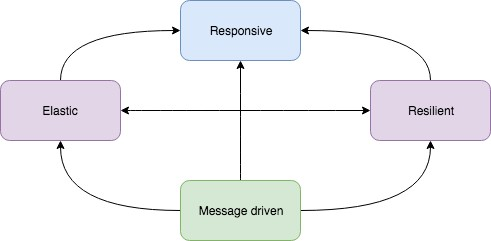
\includegraphics[width=1\textwidth]{reactive}
 \label{fig:responsive}
\end{figure}

\paragraph{Responsive}
The system responds in a timely manner if at all possible. Responsiveness means that problems may be detected quickly and deal with it effectively. 
Characteristics:
\begin{itemize}
    \item Cornerstone of usability;
    \item Systems must respond in a fast and consistent fashion if at all possible;
    \item Responsive systems build user confidence.
\end{itemize}

\paragraph{Resilient}
The system stays responsive in the face of failure. This applies not only highly-available, mission-critical systems -- any system that is not resilient will be unresponsive after a failure. Attributes:
\begin{itemize}
    \item Provides responsiveness, despite failures;
    \item Achieved through replication, isolation, containment, delegation;
    \item Failure are isolated to a single component;
    \item Recovery is delegated to an external component (If you're the failing component, then you're not reliable enough to handle your own failure. If the system goes down it can't restart itself. So an external component is needed to monitor it and restart if necessary.). 
\end{itemize}

\paragraph{Elastic}
The system stays responsive under varying workload. Reactive Systems can react to changes in the input rate by increasing or decreasing the resources allocated to service these inputs. 

\begin{itemize}
    \item Provides responsiveness, despite increase/decrease in load;
    \item Implies zero contention and no central bottlenecks. (As a directive because it's impossible in a real scenario);
    \item Predictive auto scaling techniques can be used to support elasticity;
    \item Scaling up provides responsiveness during peak, while scaling down improving cost effectiveness. 
\end{itemize}

\paragraph{Message Driven}
Reactive Systems rely on asynchronous message-passing to establish a boundary between components that ensures loose coupling, isolation and location transparency. This boundary also provides the means to delegate failure as messages.
\begin{itemize}
    \item Responsiveness, Resilience and Elasticity are all supported by a Message Driven architecture;
    \item Messages are asynchronous and non-blocking;
    \item Provides Loose coupling, isolation, location transparency;
    \item Resources are consumed only while active, meaning you don't have a situation where you make a request and that request is blocking, and you're stuck waiting for a response from someone who could take a long time getting back, or not respond back at all. While you're waiting, you're consuming any number of physical resources, threads, CPU cycles etc;
    \item Send message and release the resource. Response will then come back asynchronously.
\end{itemize}

Employing explicit message-passing enables load-management, elasticity, and flow control by shaping and monitoring the message queues in the system applying back-pressure when necessary. Location transparent messaging as a means of communication makes it possible for the management of failure to work with the same constructs and semantics across a cluster or within single host. Non-blocking communication allows recipients to only consume resources while active, leading to less system overhead.

\subsection{Goals}
The main goals to use Reactive Systems are:
\begin{itemize}
    \item Scales from 10 to 10 million users;
    \item Consumes only the resources necessary to support the current load;
    \item Handles failures with little to no effect on the user;
    \item Can be distributed across tens, hundreds, or even thousands of machines;
    \item Maintains a consistent level of quality and responsiveness despite failures.
\end{itemize}

\section{Reactive Systems vs Reactive Programming}
Reactive systems can be implemented using reactive programming or not. Reactive Systems are related to an architectural style that allows multiple individual applications to coalesce as a single unit, reacting to its surroundings, while remaining aware of each other. 

Reactive Programming is a subset of asynchronous programming and a paradigm where the availability of new information drives the logic forward rather than having control flow driven by a thread-of-execution.

\begin{itemize}
    \item Reactive Programming can be used to support the construction of Reactive Systems;
    \item It supports breaking problems into small, discrete steps that are executed in an asynchronous/non-blocking fashion, usually via a callback mechanism (Futures/Promises, Streams, RxJava, RxScala);
    \item A system that uses Reactive Programming is not necessarily a Reactive System (You could build a system with reactive programming techniques and then deployed onto a single node. It's not a reactive system because if this node crashes, the whole system will be down).
\end{itemize}

\section{Actor Model}
The actor model is a conceptual model to deal with concurrent computation. It defines some general rules for how system's components should behave and interact with each other. Characteristics:
\begin{itemize}
    \item Programming paradigm that supports the construction of Reactive Systems;
    \item Just because you use the Actor Model, doesn't mean that you've built a Reactive System;
    \item It's Message Driven, all communication is asynchronous and non-blocking;
    \item Provides abstractions that give us Elasticity and Resilience;
    \item It can therefore be used to build Responsive software;
    \item On the JVM, the Actor Model is implemented with Akka\footnote{It's what we are using to produce reactive applications. There is other solutions. As an alternative you can take a look at \href{http://scalecube.io/}{scalecube}.}.
    \item All computation occurs inside of Actors;
    \item Each actor has an address;
    \item Actors communicate only through asynchronous messages.
\end{itemize}

\subsection{Location Transparency}

\begin{figure}[ht]
\caption{Actor model location transparency}
\centering
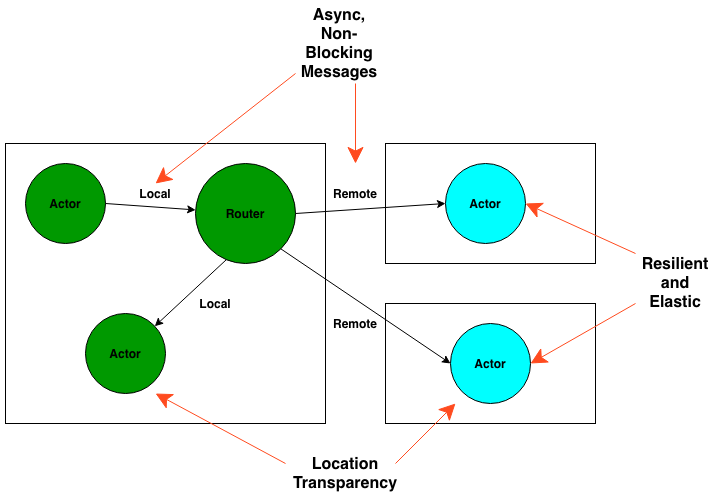
\includegraphics[width=1\textwidth]{location_transparency}
 \label{fig:location_transparency}
\end{figure}

Everything in Akka is designed to work in a distributed setting: all interactions of actors use purely message passing and everything is asynchronous. The key for enabling this is go to from remote to local by way of optimization instead of trying go from local to remote by way generalization. In summary:
\begin{itemize}
    \item Message Driven nature of Actors supports Location Transparency (Figure~\ref{fig:location_transparency});
    \item Actors communicate using the same technique, regardless of location;
    \item Local vs Remote is mostly configuration (Configure that a particular router can route to these routees. Communication mechanisms don't change at all). Original actor sends message with no knowledge of location of where that message is going to;
    \item No specific technique of API to send to a remote actor. API is identical for Remote and Local;
    \item Location transparency enables actors to be Resilient and Elastic (Resilient because we can deploy actors across multiple nodes and elastic because if we have high load, we can add more routees on more pieces of hardware, or remove to scale down.).
\end{itemize}

You can find more information about Remote vs Local transparency in the Table~\ref{tab:loctransparency}

\begin{table}[ht]
  \begin{center}
    \caption{Location transparency vs Transparent Remoting}
    \label{tab:loctransparency}
    \begin{tabularx}{\textwidth}{|Y|Y|} \hline 
      \textbf{Location Transparency} & \textbf{Transparent Remoting}\\\hline\hline
       Remote calls look like local calls. & Local calls look like remote calls.\\\hline
       Hides the fact that you're making remote calls. & Assumes you're always doing remote calls.\\\hline
       Hides potential failure scenarios (E.g. Network failures). For example, because it will look like a local call, you might not think to deal with that possibility. & You have to assume remote failure scenarios can occur (E.g. Network failures).\\\hline
    \end{tabularx}
  \end{center}
\end{table}

\paragraph{Importance of the Actor Model}
There are other reactive tools but most of them only support part of the Reactive Principles. So to achieve that you need to combine different technologies to build a Reactive System. Generally if you build a Reactive System without Actors you will probably need:
\begin{itemize}
    \item Service Registry;
    \item Load Balancer;
    \item Message Bus.
\end{itemize}

In contrast with the Actor Model can be reactive at the level of actors. So if you build you system based on actors and micro services this should be enough.
The actor model facilitates the the design of Reactive design because:
\begin{itemize}
    \item It's Message Driven by default;
    \item It's location transparent providing Elasticity and Resilience through distribution;
    \item It's Responsive because of the previous two points; (Take a look at the Figure~\ref{fig:responsive}). 
\end{itemize}

\section{References}

\begin{thebibliography}{9}

\bibitem{reactive_manifesto} 
\href{https://www.reactivemanifesto.org/}{\textit{Reactive Manifesto}}, 2014.

\bibitem{reactive_arch_1} 
Wade Waldron, 
\href{https://academy.lightbend.com/courses/course-v1:lightbend+LRA-IntroToReactive+v1/about}{\textit{Reactive Architecture(1): Introduction to Reactive Systems}}, Lightbend 2020.

\bibitem{reactive_prog_sys} 
Jonas Bon\'er and Viktor Klang,
\href{https://www.lightbend.com/blog/white-paper-understanding-reactive-programming-vs-reactive-systems}{\textit{Reactive Programming versus Reactive Systems}}, Lighbend 2020.

\bibitem{reactive_explained}
Grace Jansen and Peter Gollmar,
\href{https://www.ibm.com/downloads/cas/YEEQBXND}{\textit{Reactive Systems Explained: Jump-Start Your Journey to Reactive Architecture}}, 
IBM 2020
\end{thebibliography}
